\chapter{Evaluation} % Main chapter title

\label{Chapter6} % For referencing the chapter elsewhere, use \ref{Chapter1} 

\lhead{Chapter 5. \emph{Evaluation}}
This chapter evaluates the approach presented in Chapter \ref{Chapter3} to answer the proposed research questions. Section \ref{evalsetup} introduces the candidates selected for the empirical evaluation and describes the experimental setup. Section \ref{expeval} presents the results of the experimental evaluation.  

\section{Experimental Setup}
\label{evalsetup}
For the evaluation of the proposed approach, our goal was to select candidates that satisfy the project requirements described in Section \ref{selectingCandidates}. Unfortunately, not many applications are available which satisfy the aforementioned requirements and have publicly accessible Selenium test suites. In order to evaluate the research questions, five commercial-scale open-source web applications as described in Table \ref{appcandidates}, have been selected. All of these applications have several years of software development history.

Among the experimental candidates, Moodle\footnote{\url{https://moodle.org/}} is a widely used open-source Course Management System. Mozilla Addons\footnote{\url{https://addons.mozilla.org/}} web application hosts web-browser extensions. Mozilla Marketplace\footnote{\url{https://marketplace.firefox.com/}} is an online app portal for desktop and mobile platforms, while Mozilla.org\footnote{\url{https://www.mozilla.org/}} serves as the home for the Mozilla project. Our last candidate Jenkins\footnote{\url{https://jenkins-ci.org/}} is a popular open-source continuous integration tool. 
  
Each of these applications is installed as per the automated deployment process explained in Section \ref{sec:autoDeployment}. The automated deployment process ensures that the AUT is always installed to a `clean' state. As mentioned in Chapter \ref{Chapter4}, our approach considers different major and minor versions of candidate web applications. This setup allows us to evaluate small, incremental changes to the AUT in the form of minor revisions as well as  significant changes to the AUT in the form of major releases. 
Since different applications have different development and release cycles, we have considered approximately one year of development time-frame for each application. 

  \begin{table}
  \centering
  \resizebox{14.3cm}{!}{
  \begin{tabular}{l*{6}{l}r}
  % \\ 
  \hline
  Application              & Domain &  Major Versions & Minor Versions \\
  \hline
  Moodle            & Course Management System & 1 & 11  \\
  Marketplace     & Software Apps portal  & 4 & 22   \\
  Addons           & Browser Add-ons portal & 3 & 20  \\
  Mozilla.org     & Mozilla Project Homepage & 2 & 18   \\
  Jenkins (Weekly/ LTS) & Continuous Integration tool & 4/ 4 & 12/ 23   \\
  % Jenkins  & Continuous Integration tool & 4 & 23  \\
  \hline
  \end{tabular}}
  \caption{Overview of evaluation candidate web applications}
  \label{appcandidates}
  \end{table}

The approach illustrated in Section \ref{selectingCandidates} has been followed for selecting the major and minor releases of candidate web applications. Out of the selected web applications, only Moodle classifies the releases in terms of major-minor versions. All other applications do not identify their releases in this manner. Mozilla Addons and Marketplace follow weekly release cycles. Mozilla.org does not adhere to any specific release cycle and delivers important features and bug fixes by pushing necessary commits to its version control repository. Jenkins has two different release cycles -- Long Term Support (LTS) and weekly releases. The weekly cycle releases a new Jenkins version on weekly basis and frequently introduces new features as well as bug fixes. The LTS cycle on the other hand has relatively fewer but more stable monthly releases. Both of these release lines have been considered for the evaluation, since it would be interesting to compare how does the development process of the AUT affect the results. The chosen major and minor versions for all candidate web applications are listed in Appendix \ref{AppendixA}.

Table \ref{testcandidates} gives an overview about the test-suites of these open-source web applications. Each test-suite repository has several hundreds of commits from various contributors. The instructions for running these test-suites are also provided by the respective organizations. All of the selected web applications follow the Page-object pattern for developing their Selenium test-suites. While Jenkins\footnote{\url{https://github.com/jenkinsci/acceptance-test-harness}} and Moodle\footnote{\url{https://git.in.moodle.com/tomb/functional-test-suite}} test-suites are primarily written in Java, the Mozilla Addons\footnote{\url{https://github.com/mozilla/Addon-Tests}}, Marketplace{\footnote{\url{https://github.com/mozilla/marketplace-tests}}} and Mozilla.org\footnote{\url{https://github.com/mozilla/mcom-tests}} test-suites are written in Python.
Excluding Moodle, all other test-suites have been maintained in parallel to the development of chosen web application revisions 
% for the entire duration of the experimental phase of this thesis 
(as of March 2016, Moodle and Mozilla.org test-suite repositories have been archived and are no longer actively maintained). The `Size' column in Table \ref{testcandidates} indicates the average number of tests per test-suite. Apart from Mozilla Marketplace, all other test-suites have fairly comparable sizes. For Moodle test-suite, 38 out of 45 tests are parameterized. A parameterized test denotes a test case executed with different input values. 
\begin{table}
\centering
\resizebox{8.5cm}{!}{
\begin{tabular}{l*{6}{l}r}
\hline
Test-Suite              & Language & Page-objects & Size &LOC \\
\hline
Moodle           & Java & 13 & 43 & 2103  \\
Marketplace     & Python & 12 & 10 & 981
 \\
Addons           & Python & 17  & 55 & 3335
 \\
Mozilla.org    & Python & 16 & 60 & 2419 \\
Jenkins  & Java & 35 & 52 & 8755  \\
\hline
\end{tabular}}
\caption{Overview of Selenium test-suites for candidate web applications}
\label{testcandidates}
\end{table}

We selected these tests by executing the test-suite for the major versions of each application over multiple runs and identifying the number of ``passed'' tests, as per the approach described in Section \ref{selectingCandidates}. As a consequence, these ``passed'' tests represent a subset of the total number of available tests from the chosen candidate test-suites. The reason for selecting this subset is that the test which were marked as ``failed'' were not suitable to be considered for the robustness analysis, as they did not cover the intended functionality for the major versions in the first place. 
% There could be myriad of reasons behind this behavior, which have been briefly mentioned in Section \ref{selectingCandidates} since investigation of this behavior is beyond the scope of this thesis.
Therefore, it is important to note that throughout this chapter, the data and information presented about the Selenium test-suites refers to the selected tests alone. Correspondingly, the entries in the `Page-objects' and `LOC'\footnote{Excluding comments and blank lines, using the tool CLOC (\url{cloc.sourceforge.net})} columns have been measured for these tests.

In case of Moodle, the test-suite uses JUNIT 4.10\footnote{\url{http://junit.org/}} as a testing framework. With this test-suite we encountered different results on each test-run. In other words, the number of tests passed during each run varied significantly. Upon further investigation, we discovered that each test in the test-suite depended upon a \textit{login} test method for bringing the application in the required state of a logged-in user. This test method had a \texttt{@Test} annotation, as opposed to a setup method annotation, such as \texttt{@BeforeClass}. By default, the JUNIT 4.10 based tests were executed in random and unpredictable order assigned by the Java Virtual Machine. Hence, the \textit{login} method was not always executed before other tests and this was the reason behind the difference in the test results. In order to circumvent this issue, we executed the tests with JUNIT 4.12 which allowed the \textit{login} method to be executed as a setup method. 

Each of the test-suites have been integrated with the \texttt{webmate} tool by using the \texttt{RemoteWebdriver} capabilities for the extraction of the behavioral state models, as detailed in Section \ref{stateModelExtraction}. This automated testing setup insures that the results are reproducible. 

\section{Experimental Evaluation}
\label{expeval}
This section discusses the results of the conducted experiments and presents the answers to the research questions. 

\subsubsection*{{\bfseries RQ1.} How robust are Selenium tests against changes of the application under test?}
% \subsection{Robustness of Selenium test-suites}
% \label{robustnessresults} 
To measure the robustness of Selenium tests over the version history of a web application, the implementation steps detailed in Section \ref{toolimplementation} have been followed. 
% The independent variables for this experiment are the candidate applications (major-minor versions) and the test-suites of these applications. The dependent variable is the robustness grade of the test-suite measured across the minor versions of a major release. 
For all of the applications discussed above, the
% each major version has a corresponding test-suite. This 
test-suite is executed on major as well as minor versions along with the extraction of behavioral state models. 

As detailed in section \ref{toolimplementation}, a behavioral state model captures the actions executed by the test on the AUT, such as GUI element locators. Table \ref{testsuitedistri} gives an overview of the composition of the selected candidate test-suites. The composition can be further divided in three groups of the building blocks of the test-suite -- the type and number of GUI element locators used, number of \texttt{wait} commands implemented and the number of primary \texttt{webdriver} actions emulated within the test-suite. Since each major version has a corresponding test-suite version, the columns in Table \ref{testsuitedistri} represent the average number of entries for all test-suites of each application.  


\newcommand*\rot{\rotatebox{90}}
% \newcommand*\OK{\ding{51}}
\begin{table} [ht]
\centering
% \begin{tabular}{@{} cl*{12}c @{}}
\begin{tabular}{cl*{12}c}
%         & & \multicolumn{8}{c}{GUI Element Locators} & \multicolumn{4}{c}{Actions emulated on AUT}\\[2ex]
% \hline
        & Application & \rot{\textit{id}} & \rot{\textit{xpath}} & \rot{\textit{cssSelector}} & \rot{\textit{name}} & \rot{\textit{tagName}} & \rot{\textit{className}} & \rot{\textit{linkText}} & \rot{\textit{partialLinkText}} &  \rot{\textit{waits}} & \rot{\textit{sendKeys}}  & \rot{\textit{gets}} & \rot{\textit{clicks}}  \\
%         \cmidrule{2-12}
\hline
		& Moodle             & 10  & 59  & 15  & 0  & 0  &  0 &  1 & 1  & 170 & 90& 6  & 177 \\
        & Marketplace        & 5   & 0   & 32  &  0 &  1 &   1&  0 &  0  &  30 & 10& 12  & 22\\
        & Addons             & 12  & 5   & 94  &  0 &   0&   0& 0  &  0  &   25& 20&56  & 44\\
        & Mozilla.org        & 33  & 0   & 180  &  0 &   0&  0 &  0 & 0  &  6 & 2&66  & 60\\
        & Jenkins            & 0   & 130  &  100  & 4  &  1 & 0  &  0 & 0  &104 &200 & 280  & 430  \\
        \hline
%         \cmidrule[1pt]{2-12}
\end{tabular}
  \captionsetup{justification=justified,
singlelinecheck=false}
\caption{Statistical overview of the test-suite composition for candidate web applications. The first eight columns show the distribution of GUI Element locators. The ninth column shows the number of \texttt{wait} commands. The last three columns show the total number of \texttt{webdriver} actions emulated within each test-suite. In case of multiple major versions of the AUT, the entries in all columns represent the average number for all major version test-suites.}
\label{testsuitedistri}
\end{table}

% Therefore, a same GUI element locator-value pair (e.g. \texttt{findElement {using="id", value="uname"}}) from a page-object can be used for executing different actions in different tests. The behavioral state model captures each and every occurrence of the GUI element locator-value pair. To represent the number of GUI element locators faithfully in case of multiple occurrences, only unique GUI element locator-value pairs has been considered. 

  
The robustness grades of the test-suites for the minor versions of each major version have been measured using the definitions in Section \ref{robustnessOfSeleniumTests} for all candidate applications. Figure \ref{fig:robustnessplots} reveals how a test-suite's robustness changes over the number of software revisions. In all graphs, each point on x-axis represents a software revision. The black dots denote the robustness grade of the test-suite ($R_{TS_{V_{0}V_{i}}}$) for each minor version \textit{`i'} measured against its major version. The robustness grade lies in the interval [0.0,1.0]. Recalling from Chapter \ref{Chapter3}, the robustness grade of a test-suite for a minor version indicates the ratio of the number of robust tests for that version to the number of robust test for a reference (major) version. A value of robustness equal to 1.0 indicates that the test-suite is robust and that it can achieve the same functional coverage across the minor version as it does for the reference version; such a test-suite can be considered fit for regression testing. As mentioned in Section \ref{robustnessOfSeleniumTests}, there is a different test-suite for each major version, hence the robustness grade for each major version as a software revision corresponds to 1.0. The line drawn through the black dots reflects the overall robustness trend while the dashed vertical lines (black color) on the x-axis indicate the major version(s) of an application. Table \ref{testcandidates} provides the information regarding the size of each test-suite (average number of tests).

As depicted in Figure \ref{fig:robustnessplots}, for all the candidate web applications the robustness of test-suites appears to decline to a certain extent as newer software revisions are introduced over time. Depending upon the application and the underlying Selenium test-suites, the reasons behind the changes in the robustness vary accordingly, which are discussed in subsequent paragraphs. 

\begin{figure}[!htbp] 
\centering     %%% not \center
\vspace{-3mm}\subfigure[Moodle]{\label{rob:moodle}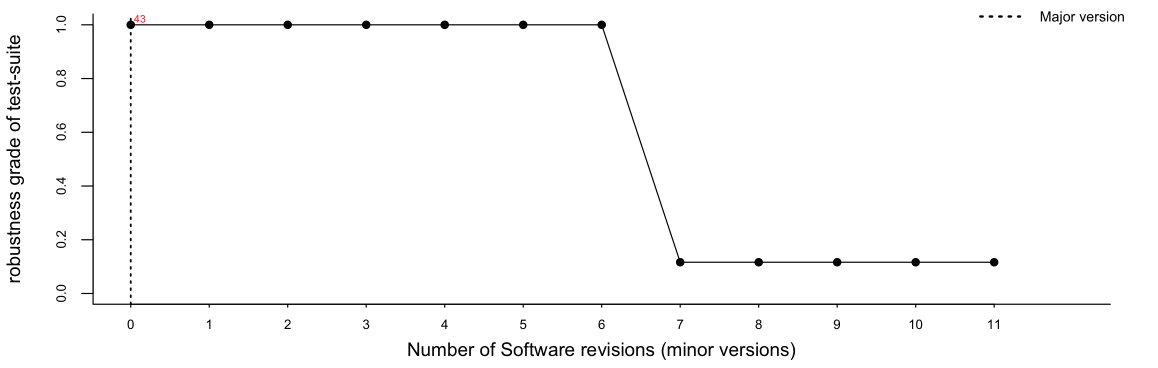
\includegraphics[width=13cm,height=3.05cm]{./Figures/moodle-rq1}}
\vspace{-2mm}\subfigure[Mozilla Marketplace]{\label{rob:fireplace}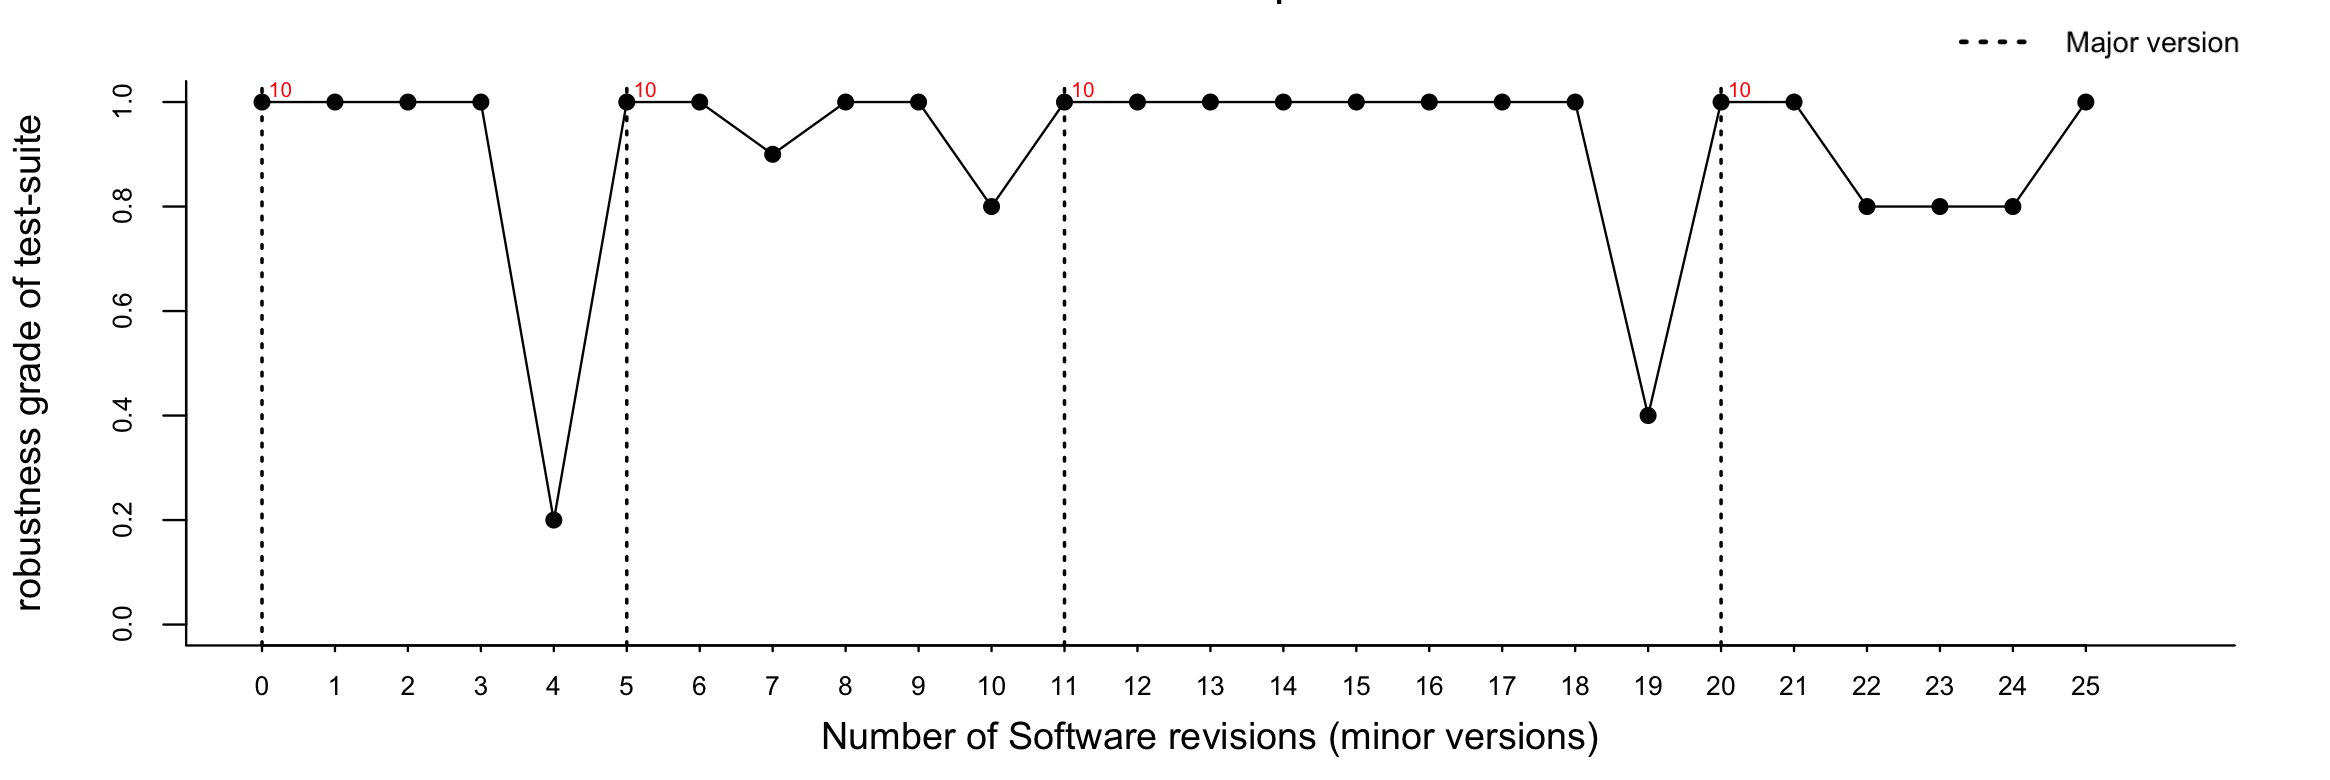
\includegraphics[width=13cm,height=3.05cm]{./Figures/fireplace-rq1}}
\subfigure[Mozilla Addons]{\label{rob:amo}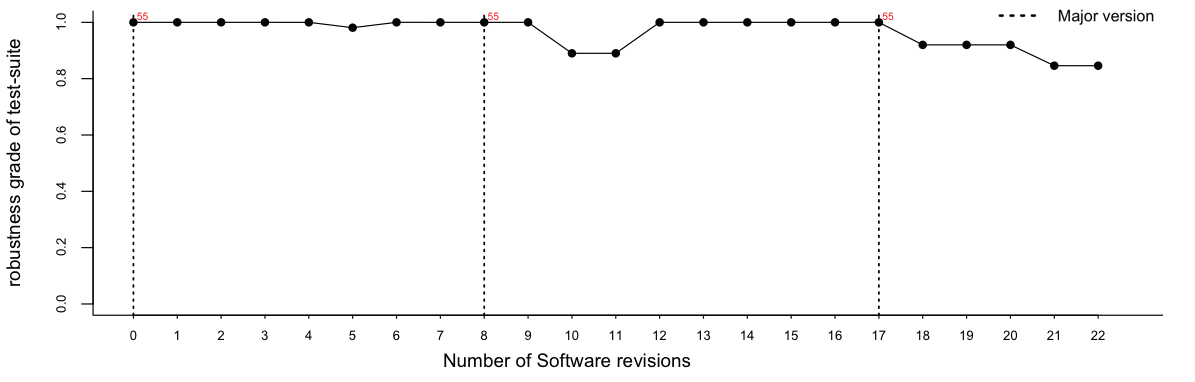
\includegraphics[width=13cm,height=3.05cm]{./Figures/amo-rq1}}
\vspace{-2mm}\subfigure[Mozilla.org]{\label{rob:bedrock}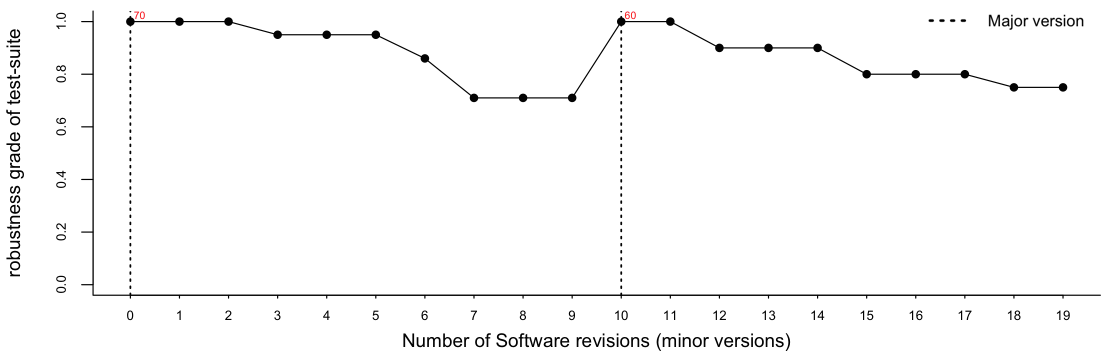
\includegraphics[width=13cm,height=3.05cm]{./Figures/bedrock-rq1}}
\captionsetup{justification=justified,
singlelinecheck=false}
\vspace{-2mm}\subfigure[Jenkins LTS Release Line]{\label{rob:LTS}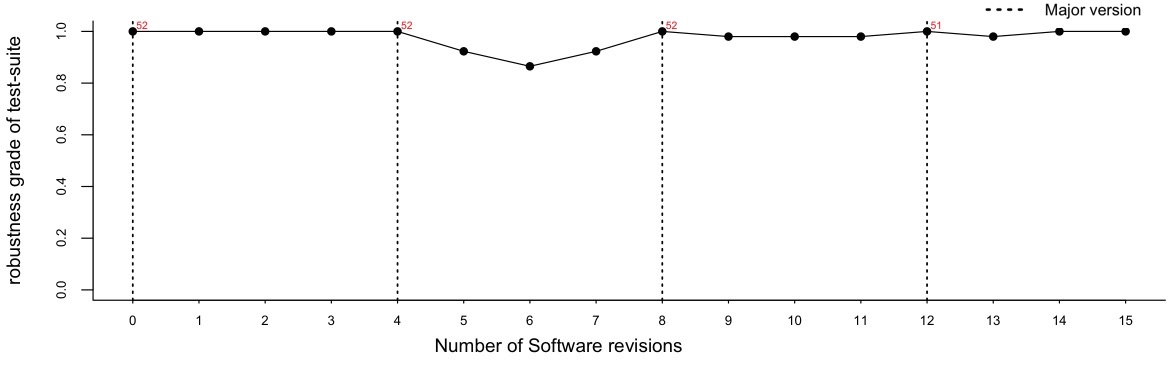
\includegraphics[width=13cm,height=3.05cm]{./Figures/jenkinsLTS-rq1.png}}
\vspace{-2mm}\subfigure[Jenkins Weekly Release Line]{\label{rob:weekly}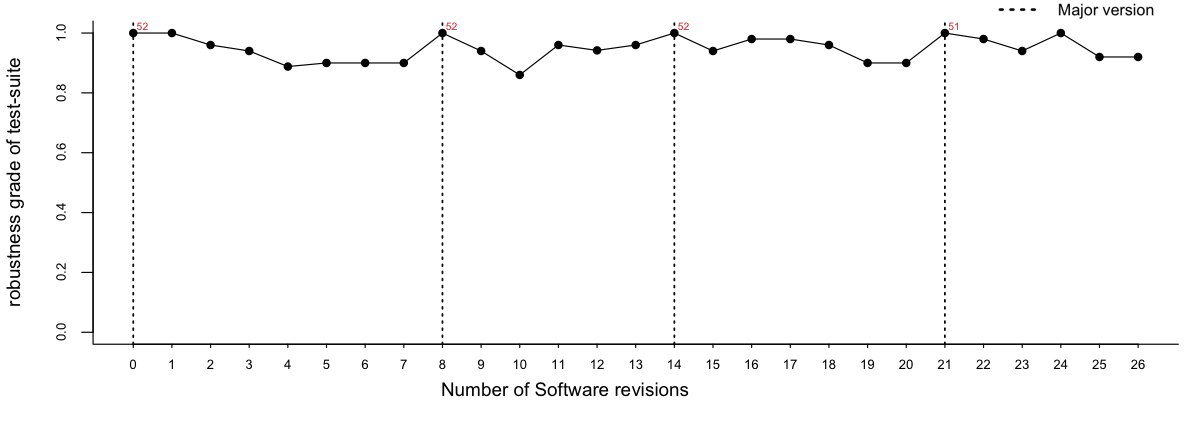
\includegraphics[width=13cm,height=3.05cm]{./Figures/jenkinsWeekly-rq1.png}}
  \captionsetup{justification=justified,
singlelinecheck=false}
\caption{Robustness trend across different revisions of candidate web applications. The x-axis represents software revisions (approximately one year of development history). The dashed vertical line represents major versions. The y-axis represents the robustness grade of the test-suite.}
\label{fig:robustnessplots}
\end{figure} 

A closer look at Figure \ref{rob:moodle} shows that out of all the applications, the robustness grade for Moodle declines the most -- almost 90\% tests were broken from seventh software revision onward. Upon investigation, it was observed that all of these tests used on \texttt{xpath} expressions to locate the \texttt{HTML} title attributes of the \textit{anchor} elements. 
Figure \ref{fig:moodleDOM} depicts this change in the structural markup of Moodle between the sixth and seventh software revision, along with the example of missing title attribute (\texttt{title="Add a new user"}). From the seventh revision onward, the \texttt{title} attributes were unavailable and as a consequence, all the tests using \texttt{xpath} locators with \texttt{title} attributes were unable to locate these GUI elements. 
% Remembering from Section \ref{challengesSelenium}, that changes the structural markup of a web-page can affect the robustness of tests. 
% Unfortunately such changes can happen during the evolution of the AUT. 
It was also noticed that the remaining 10\% robust tests in Moodle test-suite implemented only the \texttt{id} element locators. This is probably the reason why these tests were not broken due to changes in the \texttt{HTML} attributes of the page.
% Upon investigation, it was observed that  due to unavailable \texttt{xpath} expressions (\texttt{NoSuchElementException - xpath}). 
% Remembering from Section \ref{challengesSelenium}, that changing the structural markup of a web-page can affect the robustness of tests. 

% Another 

% \begin{table} 
% \centering
% \begin{tabular}{@{} cl*{12}c @{}}
% %         & & \multicolumn{10}{c}{Test-suite composition} \\[2ex]
% % \hline
%         & & \rot{\textit{id}} & \rot{\textit{xpath}} & \rot{\textit{cssSelector}} & \rot{\textit{name}} & \rot{\textit{tagName}} & \rot{\textit{className}} & \rot{\textit{linkText}} & \rot{\textit{partialLinkText}} & \rot{\textit{sendKeys}} & \rot{\textit{waits}} & \rot{\textit{gets}} & \rot{\textit{clicks}}  \\
% %         \cmidrule{2-12}
% \hline
% 		& Moodle             &w&   &   &   &   &   &  &   &   &  & &w \\
%         & Marketplace               &  &  &  &  &  &  &  &  &  &  & & \\
%         & Addons              &  &   &   &   &  &  &  &   &  &  & & \\
%         & Mozilla.org  &  &  &  &  &  &   &  &  &  &  & & \\
%  \rot{\rlap{~Application}}
%         & Jenkins                & w &   &   &   &   &   &  &   &  &  & &w \\
%         \hline
% %         \cmidrule[1pt]{2-12}
% \end{tabular}
% \caption{Some caption}
% \label{testsuitedistri}
% \end{table}

\begin{figure}[ht!] 
\centering     %%% not \center
\subfigure[Moodle Revision No. 6]{\label{rob:moodleDOm1}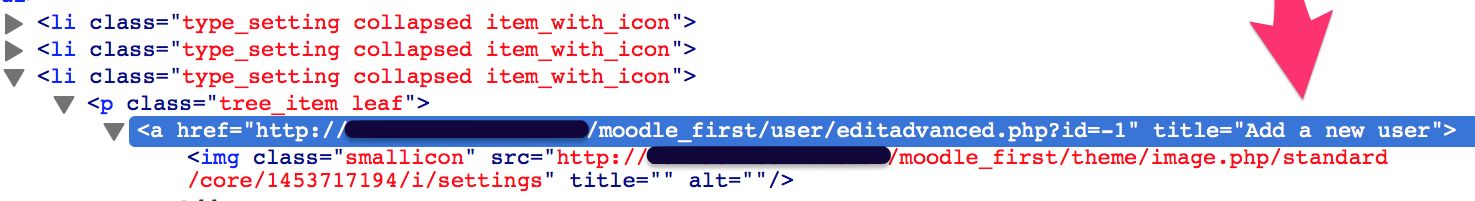
\includegraphics[width=\linewidth]{./Figures/moodle1}}
\subfigure[Moodle Revision No. 7]{\label{rob:moodleDOm2}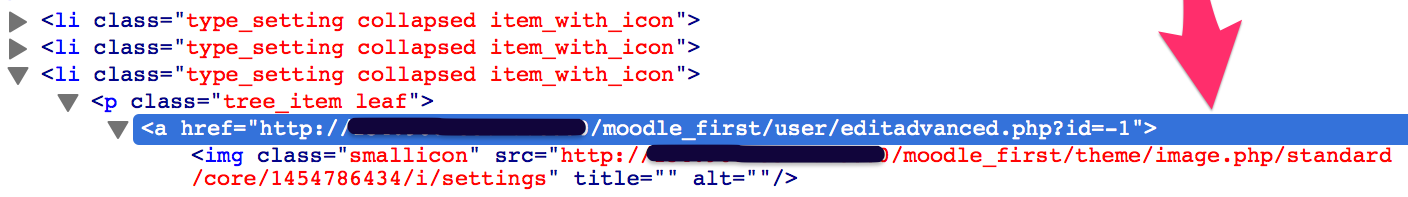
\includegraphics[width=\linewidth]{./Figures/moodle2}}
  \captionsetup{justification=justified,
singlelinecheck=false}
\caption{DOM level differences between two successive software revisions of Moodle. The red arrow highlights the missing \texttt{title="Add a new user"} in Figure (b). (Note: The URL has been stricken through for security reasons.)}
\label{fig:moodleDOM}
\end{figure} 

% Another interesting observation was in case of Mozilla Marketplace. Between the fourth and the fifth revision, the GUI of the application underwent some design changes, as depicted in Figure \ref{fig:fireplacechanges}. In this case, the tests were unable to explore the desired functionality, as they could not detect the presence of certain GUI fields before performing an action on them. As an example the `search' functionality state in the aforementioned figure was not reached in Figure \ref{rob:fire2}.



% \begin{figure}[ht!] 
% \centering     %%% not \center
% \subfigure[Marketplace Revision No. 3]{\label{rob:fire1}
\includegraphics[width=\linewidth]{./Figures/fireplace1}}
% \subfigure[Marketplace Revision No. 4]{\label{rob:fire2}
\includegraphics[width=\linewidth]{./Figures/fireplace2}}
%   \captionsetup{justification=justified,
% singlelinecheck=false}
% \caption{Changes in the GUI design between two successive software revisions of Marketplace. }
% \label{fig:fireplacechanges}
% \end{figure} 

Changing the manner in which functionality is accessed also had an effect on the robustness grade of the test-suite. As shown in \ref{fig:bedrockchanges}, between two revisions of Mozilla.org (revision six and seven), a particular `Products' page was no longer accessible through the same URL. This can happen when a certain functionality is moved to another part of the application. Clearly, due to such change the tests are not able to cover the same functionality. 

\begin{figure}[ht!] 
\centering     %%% not \center
{\label{rob:bedrock1}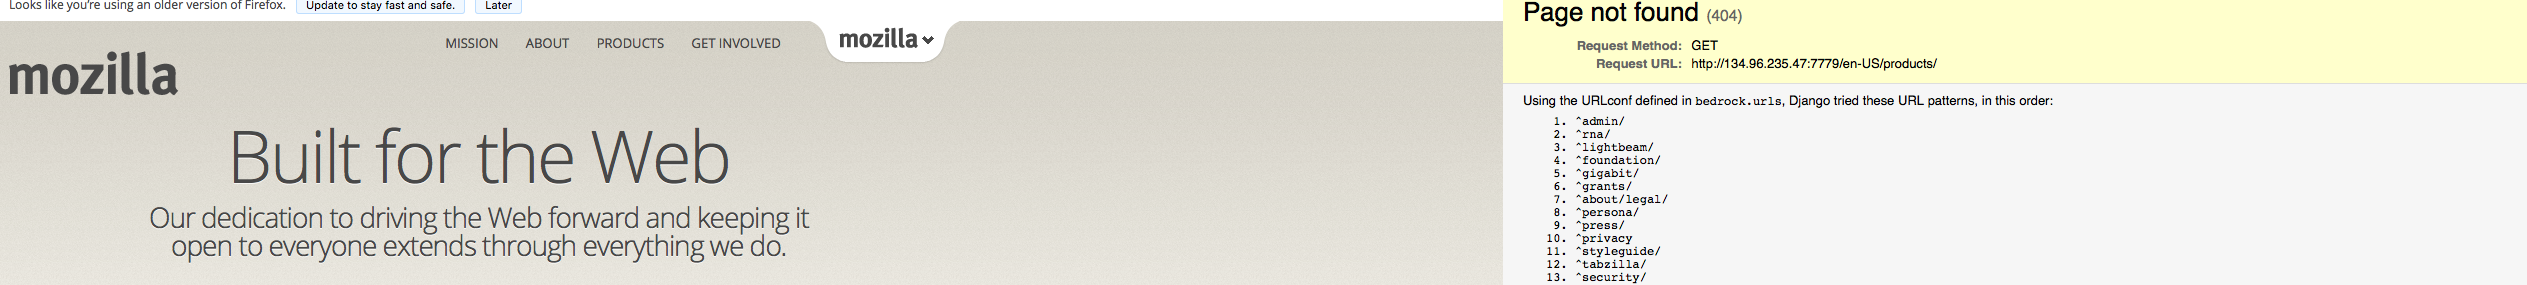
\includegraphics[width=\linewidth]{./Figures/bedrock1}}
\captionsetup{justification=justified,
singlelinecheck=false}
\caption{ The left part of the image shows the `Products' page for Revision No. 6 while the right part shows the `Products' page for Mozilla.org was no longer accessible through the same URL for Revision No. 7.}
\label{fig:bedrockchanges}
\end{figure} 

These examples can be an indication of how GUI level changes in the AUT affects the robustness of tests. Additionally, the composition of the test-suites could also have contributed towards the robustness. From Table \ref{testsuitedistri} it can be observed that for all the applications the use of \texttt{xpath, css selector} and \texttt{id} locators outnumbers the other locator types. Jenkins and Moodle test-suites use high number of \texttt{xpath} locators, while the three Mozilla test-suites primarily use \texttt{id} and \texttt{css selectors}. Although \texttt{xpath} expressions have not turned out to be as robust in case of Moodle, Jenkins test-suites implement `conditional' \texttt{xpath} expressions (as shown in Listing \ref{jenkinsxpath}) which provide the possibility of locating the same element using different methods. 

\begin{center}
\begin{scriptsize}
\centering
\lstset{
  basicstyle=\ttfamily,
  columns=fullflexible,
  keepspaces=true,
%   frame=none,
}
% \verb|basicstyle=\ttfamily, columns=fullflexible, keepspaces=true|
  
\begin{lstlisting}[caption=Jenkins conditional \texttt{xpath} expression,label=jenkinsxpath]
findElements {using="xpath", value=" .//input[@type='radio'][./@id ='Delegate to servlet container' 
or ./@name = 'Delegate to servlet container' 
or ./@value = 'Delegate to servlet container' 
or ./@placeholder = 'Delegate to servlet container']
}
\end{lstlisting}
\end{scriptsize} 
\end{center}

% As mentioned in Section \ref{stateModelExtraction}, the behavioral state model can only capture \texttt{wait} commands which have a measurable duration. Jenkins test-suite implements two kinds of \texttt{wait} commands -- implicit waits and page-load timeouts\footnote{\url{https://w3c.github.io/webdriver/webdriver-spec.html\#dfn-session-page-load-timeout}}. All other applications use implicit waits in their test-suites. In case of number of \texttt{sendKeys} inputs, the Addons, Marketplace and Mozilla.org test-suites use relatively fewer text inputs. 

The development process of the candidate applications also appears to have an effect on the robustness trend. Applications such as Jenkins LTS were relatively robust. As mentioned earlier, the LTS releases had less frequent changes and more stable development cycle. Such a development process can indicate that the Selenium tests are less susceptible to the volatility of the GUI changes in the AUT.  

!
EXAMPLES
Statistical analysis has shown that there have not been significant factors greatly contributing towards high level of robustness during the testing. This, however, is not in accordance with the fact that some tests were more successful, i.e. robust, than others. Therefore, some of the tests did actually have certain patterns in their composition that made them more effective. In order to see what exactly had contributed towards higher robustness grade, the above detected reasons for failure of the tests will be of great help. 

Not every test developers the same problems. This can be due to the different changes on AUT as well as the different approach to addressing the problem. One of the examples for a different approach has been noticed with Jenkins application, whose test-suites were able to locate the same element by using different methods, i.e. implementation of conditional xpath expression.

!


% \begin{sidewaysfigure}[ht!] 
% % \centering     %%% not \center
% \subfigure[Moodle Revision 6]{\label{rob:amo}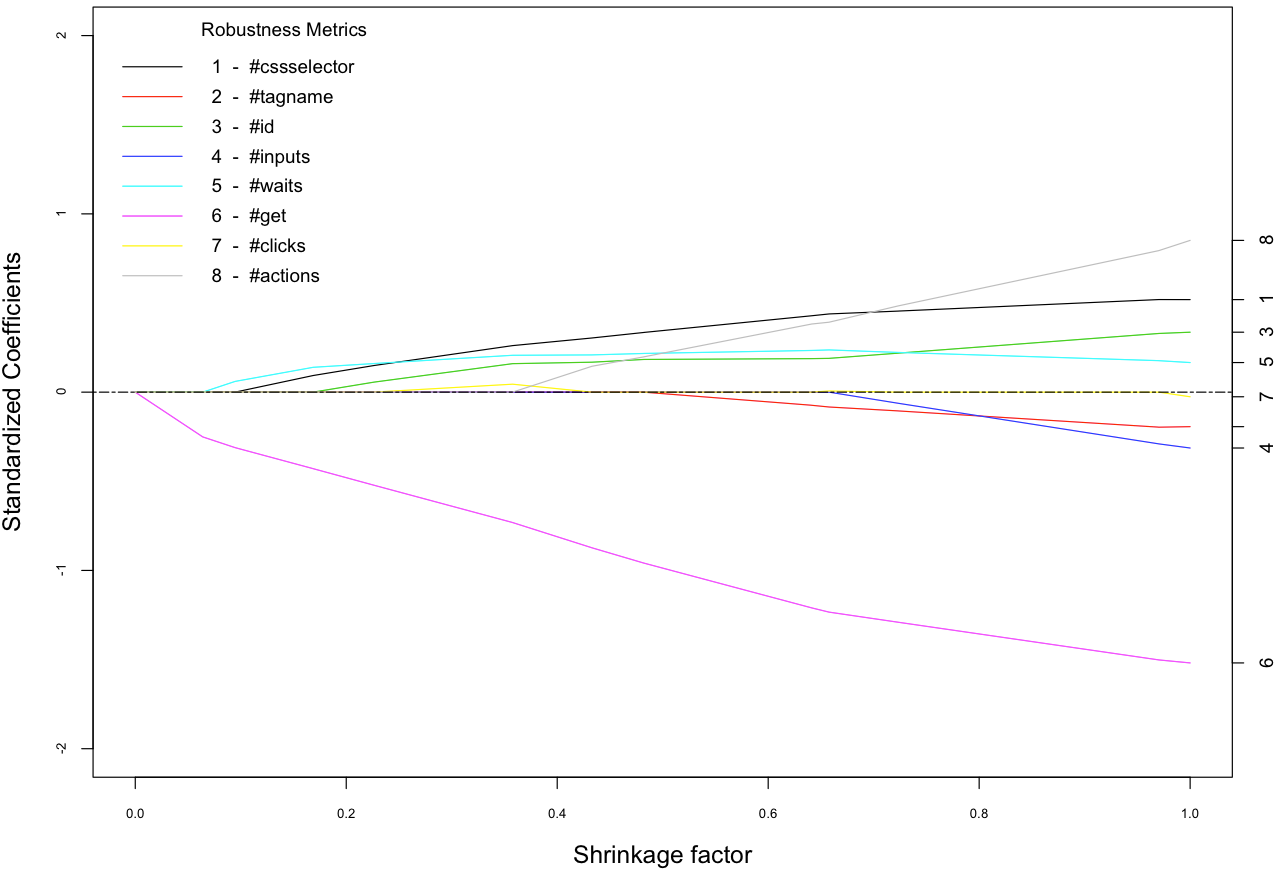
\includegraphics[width=7cm,height=6.2cm]{./Figures/fireplacelasso}}
% \subfigure[Moodle Revision 7]{\label{rob:fireplace}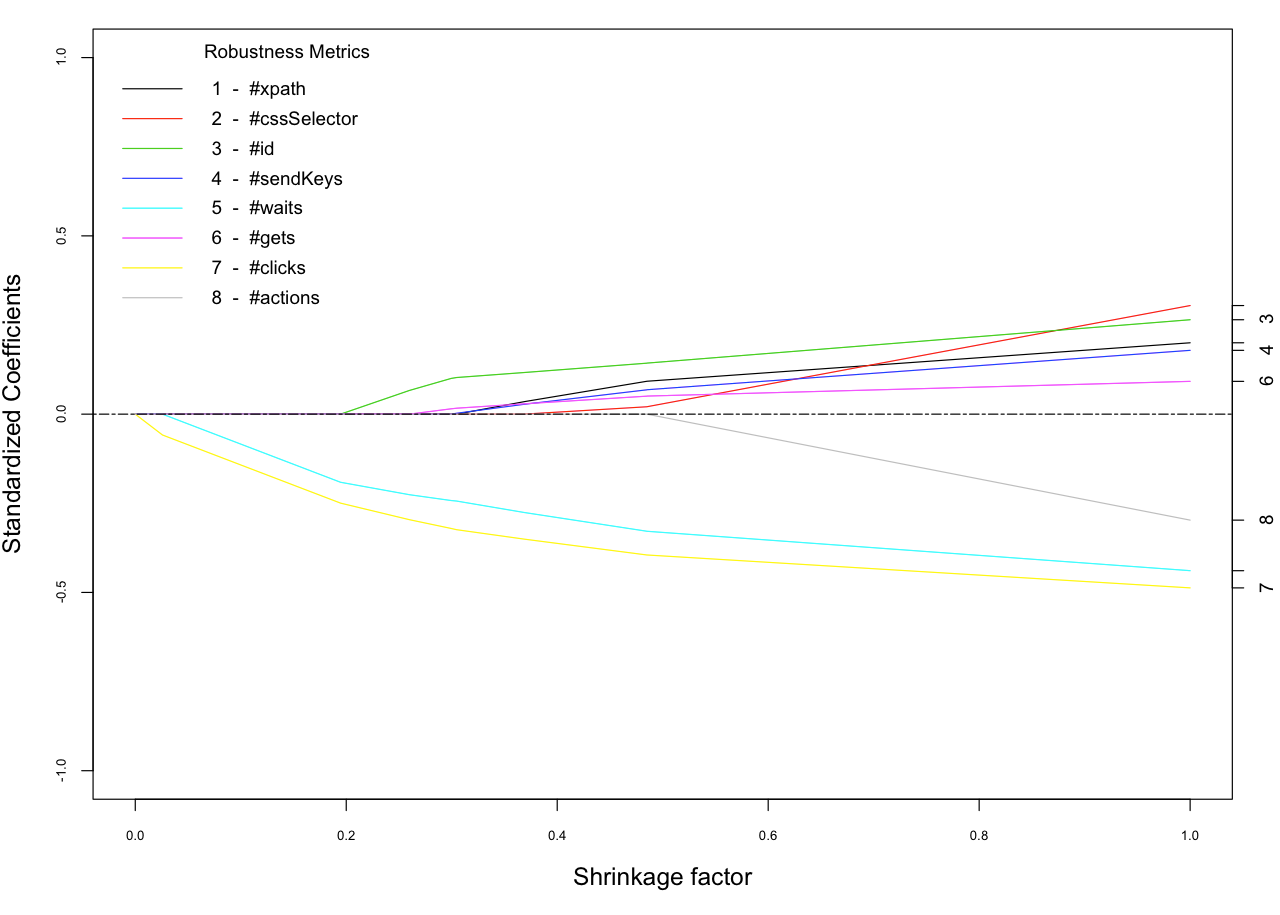
\includegraphics[width=7cm,height=6.2cm]{./Figures/amolasso}}
% \subfigure[Moodle Revision 6]{\label{rob:amo}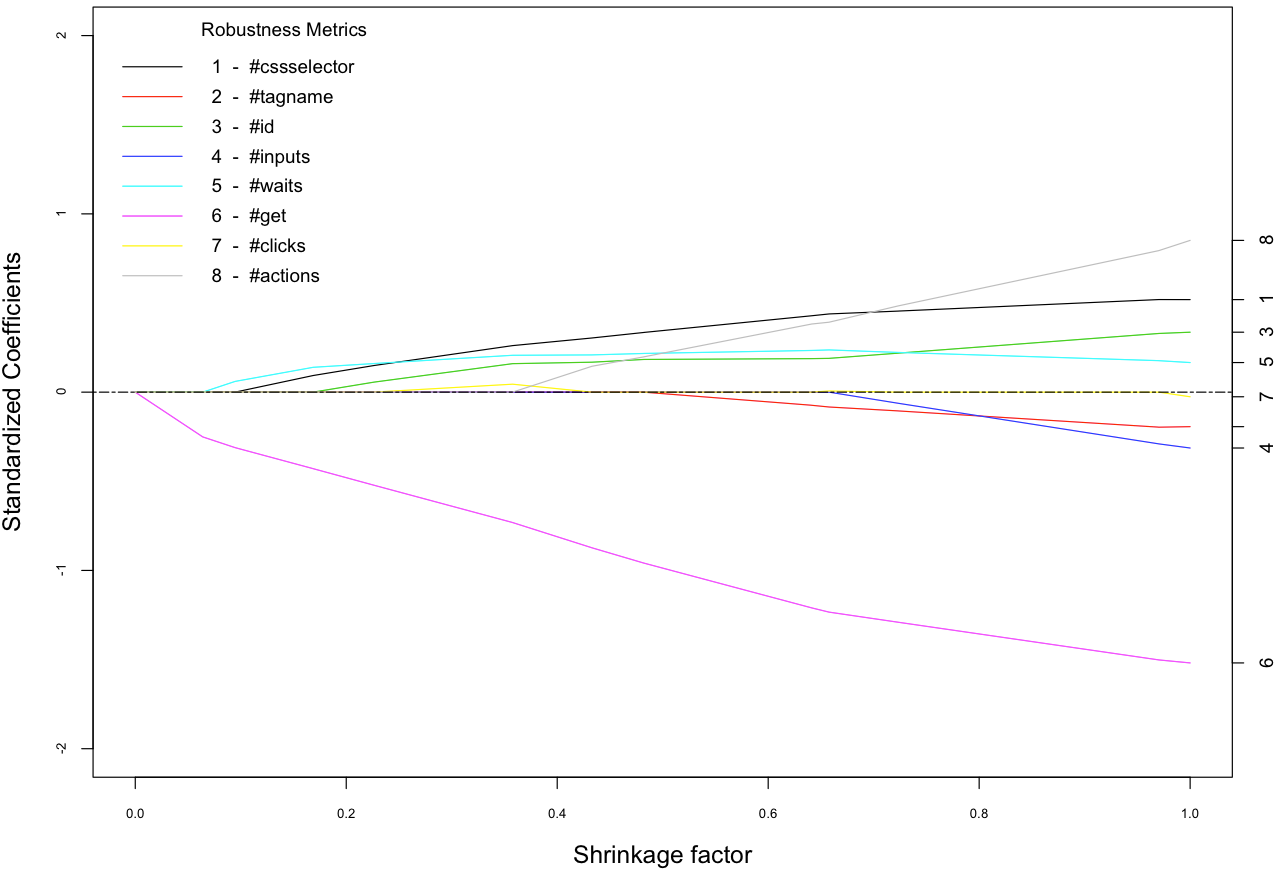
\includegraphics[width=7cm,height=6.2cm]{./Figures/fireplacelasso}}
% \subfigure[Moodle Revision 7]{\label{rob:fireplace}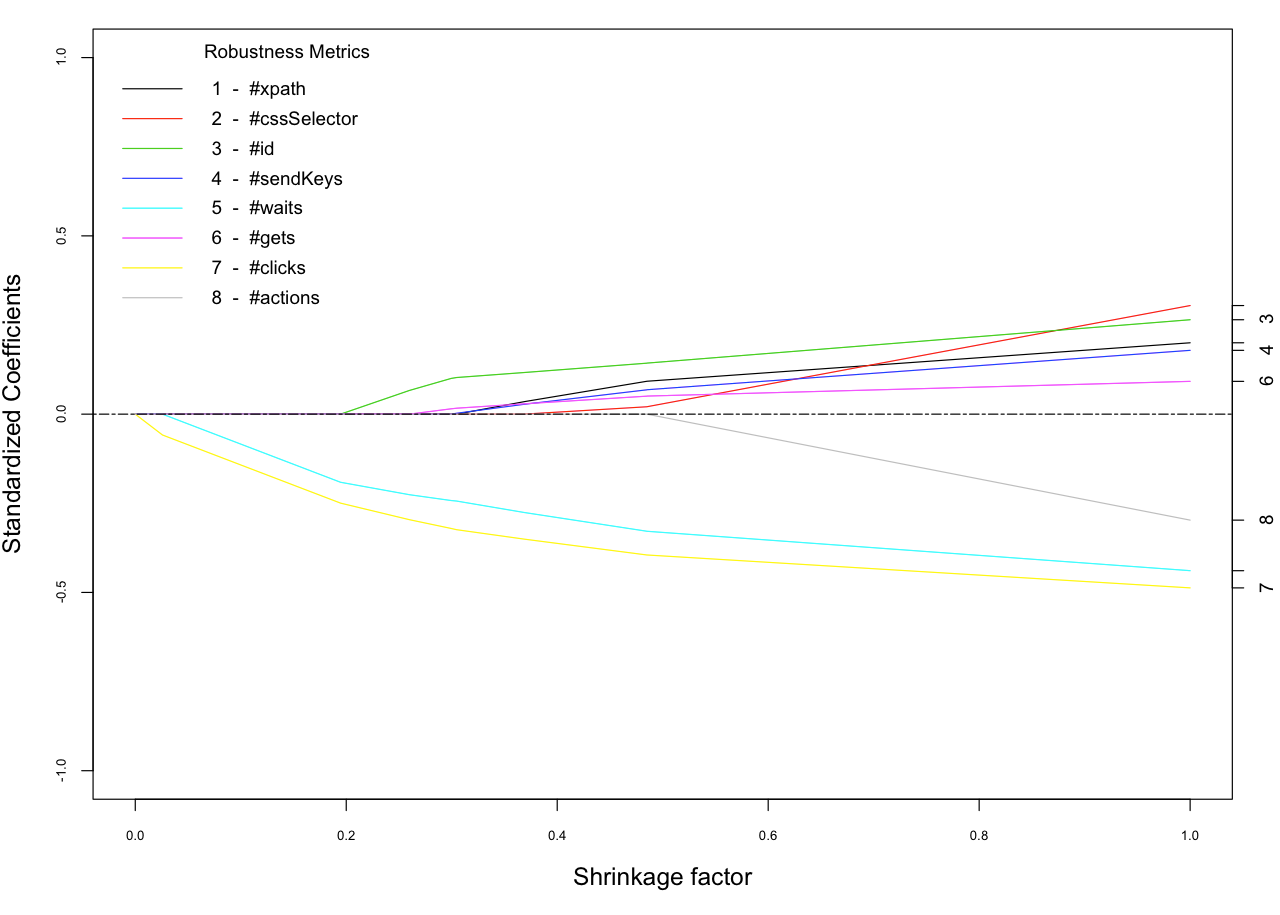
\includegraphics[width=7cm,height=6.2cm]{./Figures/amolasso}}
% \subfigure[Moodle Revision 7]{\label{rob:fireplace}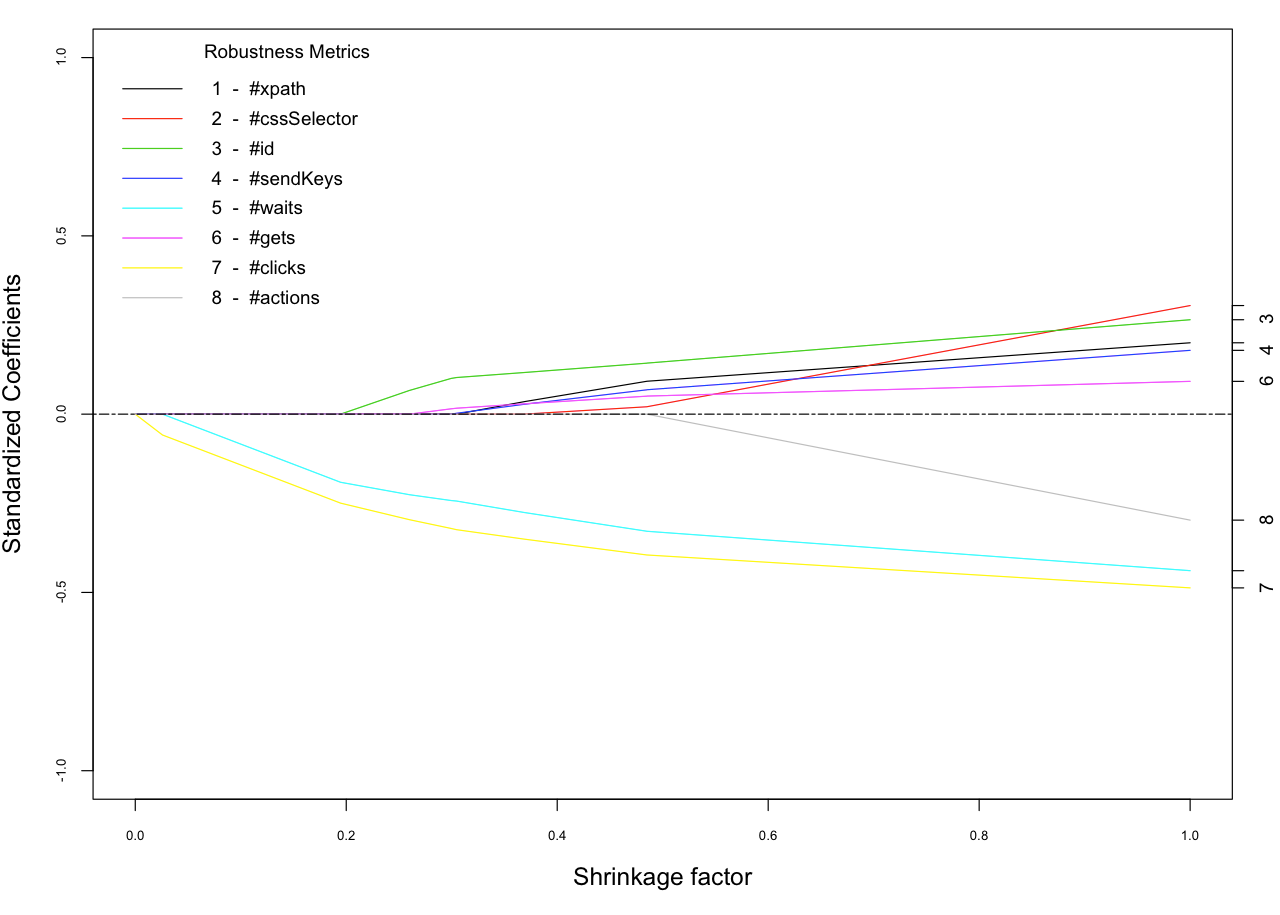
\includegraphics[width=7cm,height=6.2cm]{./Figures/amolasso}}
%   \captionsetup{justification=justified,
% singlelinecheck=false}
% \caption{DOM level differences between two successive software revisions of Moodle. The red arrow highlights the missing \texttt{title="Add a new user"} in Figure (b). }
% \label{fig:moodleDOM}
% \end{sidewaysfigure} 

\subsubsection*{{\bfseries RQ2.} Is robustness correlated to the design and composition of the tests?}

To estimate whether there is a correlation between the robustness metrics presented in in Chapter \ref{Chapter3} (Table \ref{rq2metrics}) and the robustness grade of Selenium tests, the implementation approach described in Section \ref{toolimplementation} has been followed. The robustness metrics have been extracted from the behavioral state models and the ground truth (robustness grade of a test) has been established using \texttt{webmate}. The robustness metrics are represented as a feature matrix extended with the ground truth as the solution vector, as depicted in Figure \ref{fig:featurematrix}. The metrics are the independent variables and the robustness grade is the dependent variable using which the statistical analysis has been performed.

The box plot in Figure \ref{fig:spearman} represents the Spearman rank correlation between the robustness of Selenium tests and the proposed robustness metrics which have been developed in Chapter \ref{Chapter3}. Remember that the robustness metrics represent the building blocks of a test's design and composition. The x-axis represents the robustness metrics, while the y-axis reflects the Spearman's rank correlation coefficient for candidate web applications. As mentioned in Section \ref{sec:Statistical}, a high correlation coefficient indicates that when value of one variable increases, value of other variable increases as well. While a high negative value indicates that when value of one variable increases, value of other variable decreases. A value close to zero indicates that the two variables are statistically independent. 
% It should be noted that correlation does not imply causation. 

Each box also represents the `spread' of the Spearman's correlation coefficient for each metric across the candidate applications (data sets). The horizontal lines inside the boxes represent `median' correlation coefficient. The vertical bars (`whiskers') stretching out on both sides of the box represent the `range' of the values of the correlation coefficient. The stand-alone point indicates `outlier' i.e. value which lies outside the `range' -- farther than one and half times the length of the box. 

A closer look at the box plot reveals the median correlation coefficient for most of the metrics lies between [-0.2,0.2]. The metrics \textit{\#name} and \textit{\#tagName} only have one and two coefficient values, respectively. This is due to the fact that the GUI element locator \texttt{name} is used only in Jenkins test-suite, while \texttt{tag name} locator is used only by Mozilla Marketplace and Jenkins (this can be observed in Table \ref{testsuitedistri}). Similarly, not all metrics are applicable on all applications. Metrics where the standard deviation is zero, are not included during the correlation computation. This is because a standard deviation of zero indicates that the metric has no spread (e.g. all sample values are the same) and that it would not have any influence on the dependent variable. This is the case for metrics \textit{\#partialLinkText}, \textit{\#linkText} and \textit{\#className}. As it can be observed, out of all the metrics, \textit{\#name} and \textit{\#tagName} correlation coefficients are very close to zero. This indicates that these metrics may have a very weak influence on the robustness grade. 

\begin{figure}[ht!] 
\centering     %%% not \center
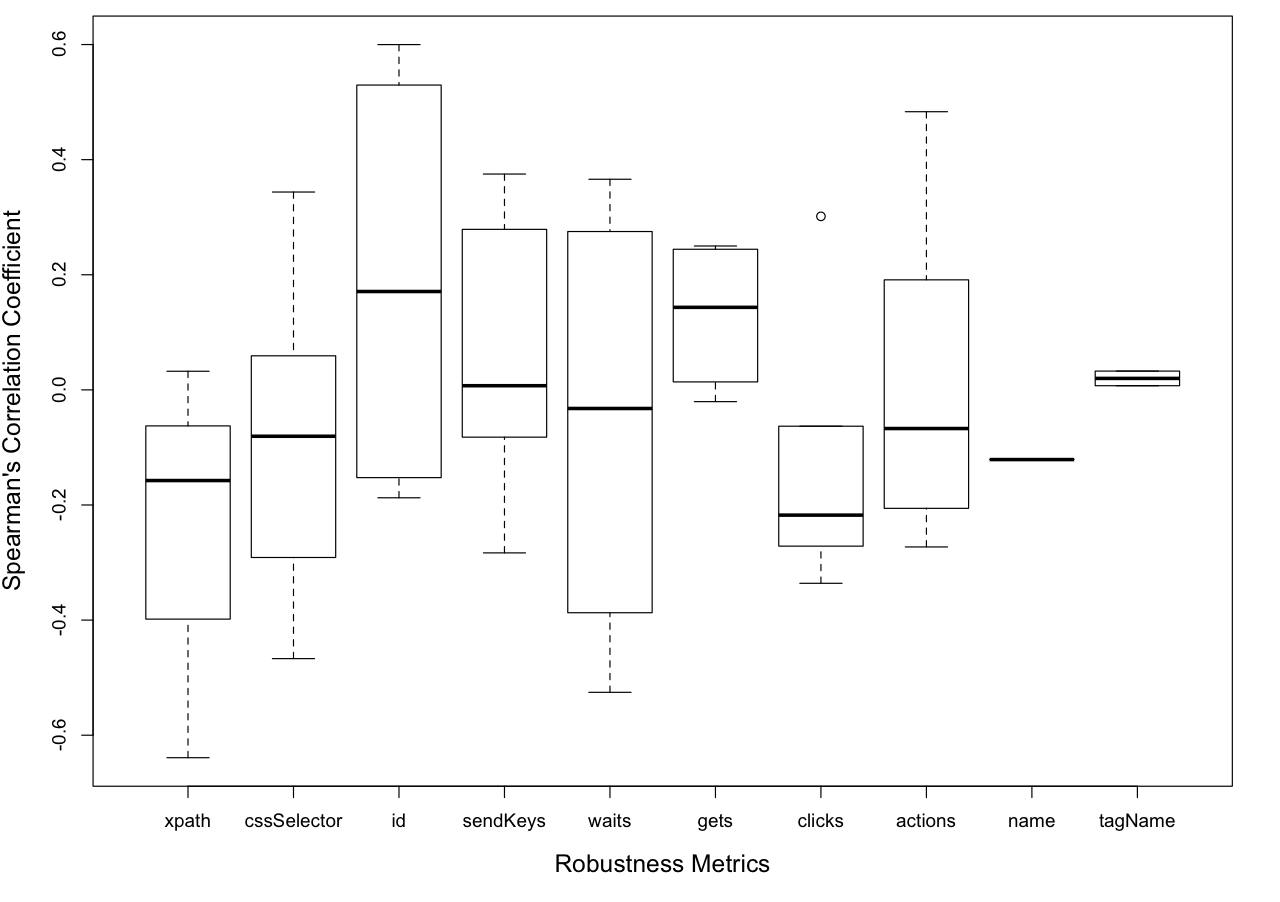
\includegraphics[width=12cm,height=8cm]{./Figures/spearman-rq2}
 \captionsetup{justification=justified,
singlelinecheck=false}
\caption{Spearman correlation box plot. The x-axis represents the robustness metrics and the y-axis represents the Spearman's correlation coefficient. (Note: For better readability, the `\#' sign has been omitted from the metrics' names.)}
\label{fig:spearman}
\end{figure} 

% \subsection{Design and Composition of tests}

In statistics, the function \textit{p-value} can be used to determine the significance of the outcome of a test. In case of correlation, a small p-value can be used as a guideline to eliminate the possibility of correlation due to random sampling. 
In the observed correlation coefficients, the metric \textit{\#xpath} has two coefficients of -0.63 (Moodle),-0.15 (Addons) which have p-values $<$ 0.005. Whereas the metric \textit{\#id} has strongest positive correlation of +0.59 with p-value $<$ 0.005. This coefficient represents the Moodle data set. Recalling from previous section, all of the tests using \texttt{id} locators in Moodle test-suite were robust. Thus, from the observed data, the \textit{\#id} and \textit{\#xpath} metrics suggest a relationship with the robustness grade.  


% In case of \textit{\#cssSelector} the two of the moderate correlation coefficients of -0.466 (Mozilla.org) and -0.29 (Moodle) have p-values $<$ 0.05. 

% For the metric \textit{\#waits} the correlation coefficient shows a high standard deviation, the p-values for positive correlation coefficients 0.36 and 0.18 are $>$ 0.2, while the p-values for negative correlation coefficients -0.52 and -0.24 are $<$ 0.001.  
% Remembering that this metric represents the number of \texttt{wait} commands in a test, a negative correlation suggests that higher number number of \texttt{wait} commands in a test might decrease its robustness. 

For metrics with large deviations in the correlation coefficients (e.g. in case of \textit{\#cssSelector, \#sendKeys, \#waits}) make it further complicated to interpret the influence the metric has on robustness grade. Two important factors affecting this behaviors are the sample size of each test-suite and the overall robustness of the tests. Consider the metric \textit{\#sendKeys} for example. For this metric the correlation coefficient of -0.28 for Addons was observed with p-value $<$ 0.005 while the correlation coefficients of 0.27 for Moodle, the p-value was $>$0.6. For both of these applications, the histograms in Figure \ref{fig:AddonsHist} and \ref{fig:moodleHist} depict the difference in the distribution of robustness grade. From previous section we remember that almost 90\% of tests for Moodle were not robust for half of the minor versions while almost 90\% of the Addons tests were robust. In such situations, a p-value may not fully indicate the strength of the rank correlation. For the remaining correlation coefficients, the observed correlation was either weak (coefficient between -0.10 to 0.10) or the p-values were high ($>$ 0.4). 

\begin{figure}[htb!] 
\centering     %%% not \center
\subfigure[Mozilla Addons]{\label{fig:AddonsHist}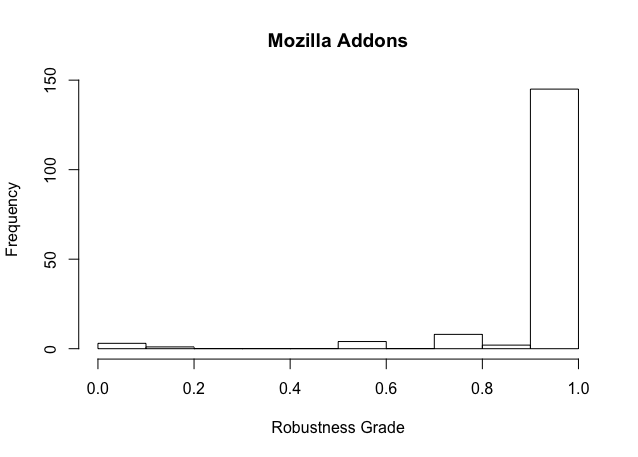
\includegraphics[width=7cm,height=5cm]{./Figures/AddonsHist}}
\subfigure[Moodle]{\label{fig:moodleHist}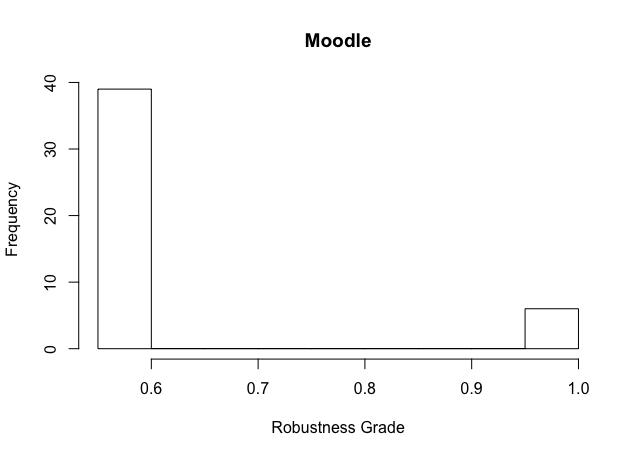
\includegraphics[width=7cm,height=5cm]{./Figures/moodleHist}}
  \captionsetup{justification=justified,
singlelinecheck=false}
\caption{Histogram distributions of robustness grade for Mozilla Addons and Moodle. The x-axis represents robustness grade and y-axis represents the frequency.}
\label{fig:hist}
\end{figure} 

A large deviation from the x-axis further indicates that for a given metric, the correlation coefficient takes negative and positive values for different applications. From the observed data, it is therefore not straightforward to determine the significance of the correlation between the metrics and the robustness grade. From what we observed in the last section, with the exception of Moodle, other test-suites were relatively robust. This implies that for majority of the tests from these test-suites, the dependent variable (robustness grade) was equal to one despite the changes in the independent variables. In this case, there are many `ties' in the ranks of the ordered variables, which can affect the computation of the correlation coefficient. 

To verify whether the above-mentioned observation is due to the ties in the ranking, we can compute the correlation coefficient which is not affected by the ties, such as Pearson's correlation coefficient. However, it should be noted that Pearson's correlation requires a linear relationship between two variables, which might not hold true for every metric. Figure \ref{fig:pearson} represents the box plot for Pearson's correlation coefficient. As we can see, the spread of the coefficients is shorter as compared to Spearman's coefficients for most of the metrics while the median values are closer to zero as compared to Spearman's coefficients. These differences can occur on account of not meeting the assumptions of Pearson's correlation (e.g. linearity) by certain variables. Overall, the distribution of the correlation coefficients do not appear to indicate any surprising differences between these two correlation methods.

\begin{figure}[ht!] 
\centering     %%% not \center
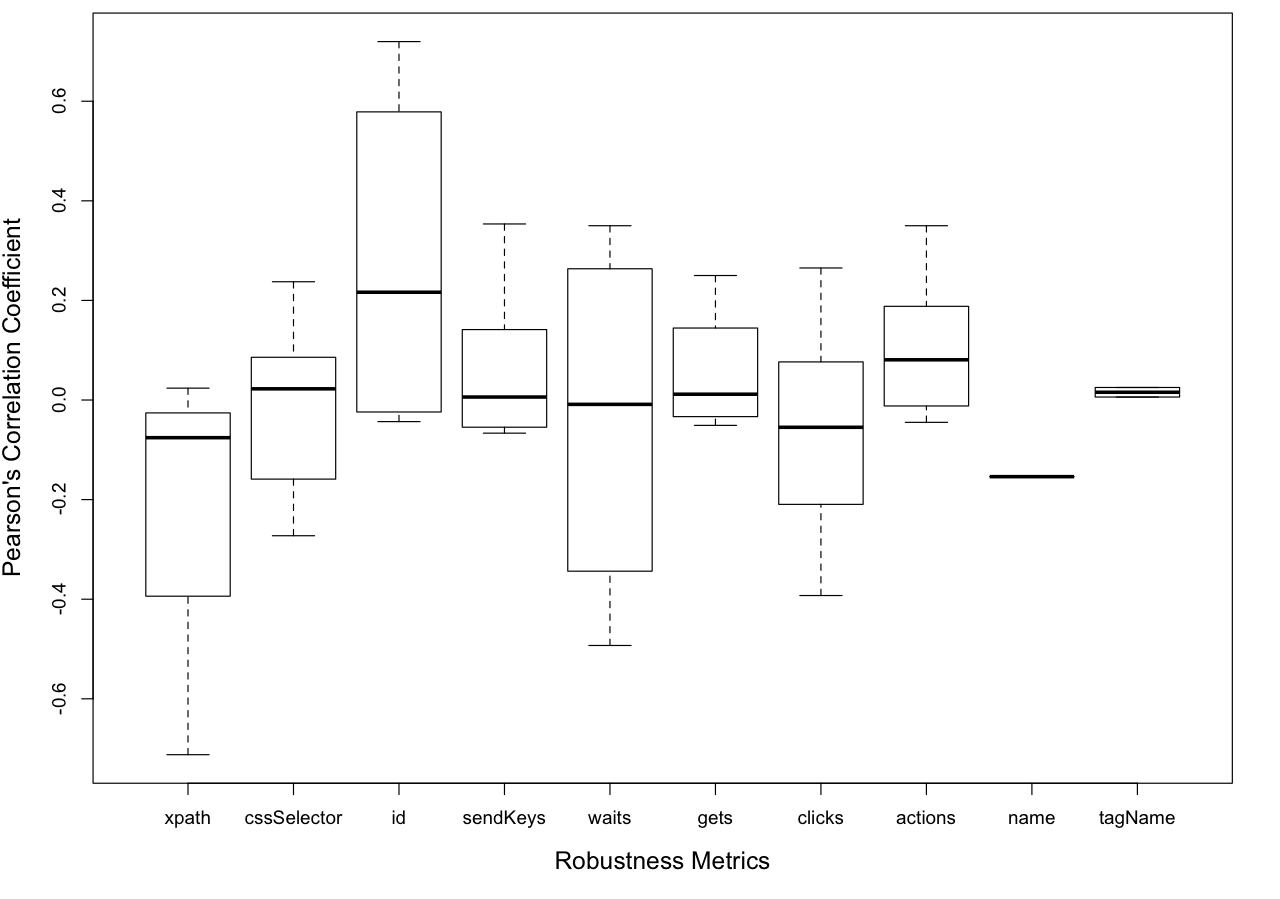
\includegraphics[width=12cm,height=8cm]{./Figures/pearson-rq2}
 \captionsetup{justification=justified,
singlelinecheck=false}
\caption{Pearson correlation box plot. The x-axis represents the robustness metrics and the y-axis represents the Pearson's correlation coefficient. (Note: For better readability, the `\#' sign has been omitted from the metrics' names.)}
\label{fig:pearson}
\end{figure}

It is also possible that some of the metrics are  strongly correlated with each other and some metrics are more meaningful to assess than others. Therefore a subset of most significant metrics can be identified. As mentioned in Section \ref{regression}, to identify the most influential metrics from the set of presented metrics the \textit{lasso} shrinkage has been applied on the data sets represented as the feature matrix and the solution vector. All the data sets for candidate applications have been standardized, as described in Section \ref{datasetstandardization}. 

Figures \ref{fig:lasso1}, \ref{fig:lasso2}, and \ref{fig:lasso3} represent the \textit{lasso} shrinkage models for candidate web applications. Each `path' on the graphs depicts a robustness metric represented by a distinct color. The x-axis represents the shrinkage factor and the y-axis represents standardized correlation coefficients of the correlation between a metric and the robustness grade. The legend on the top-left corner represents the robustness metrics.

% Recall that metric \textit{\#sendKeys} represents number of text inputs. 

% A positive correlation coefficient indicates that more the number of text inputs in a test the more robust the test was. From previous section we remember that almost 90\% of tests for Moodle were not robust for half of the minor versions while only six tests were fully robust as seen in Figure \ref{fig:moodleHist}. Hence the p-values do help to assess the strength of the correlation in this situation.





% \label{robustnessresults} 
\begin{figure}[t] 
\centering     %%% not \center
{\label{fig:moodlelasso}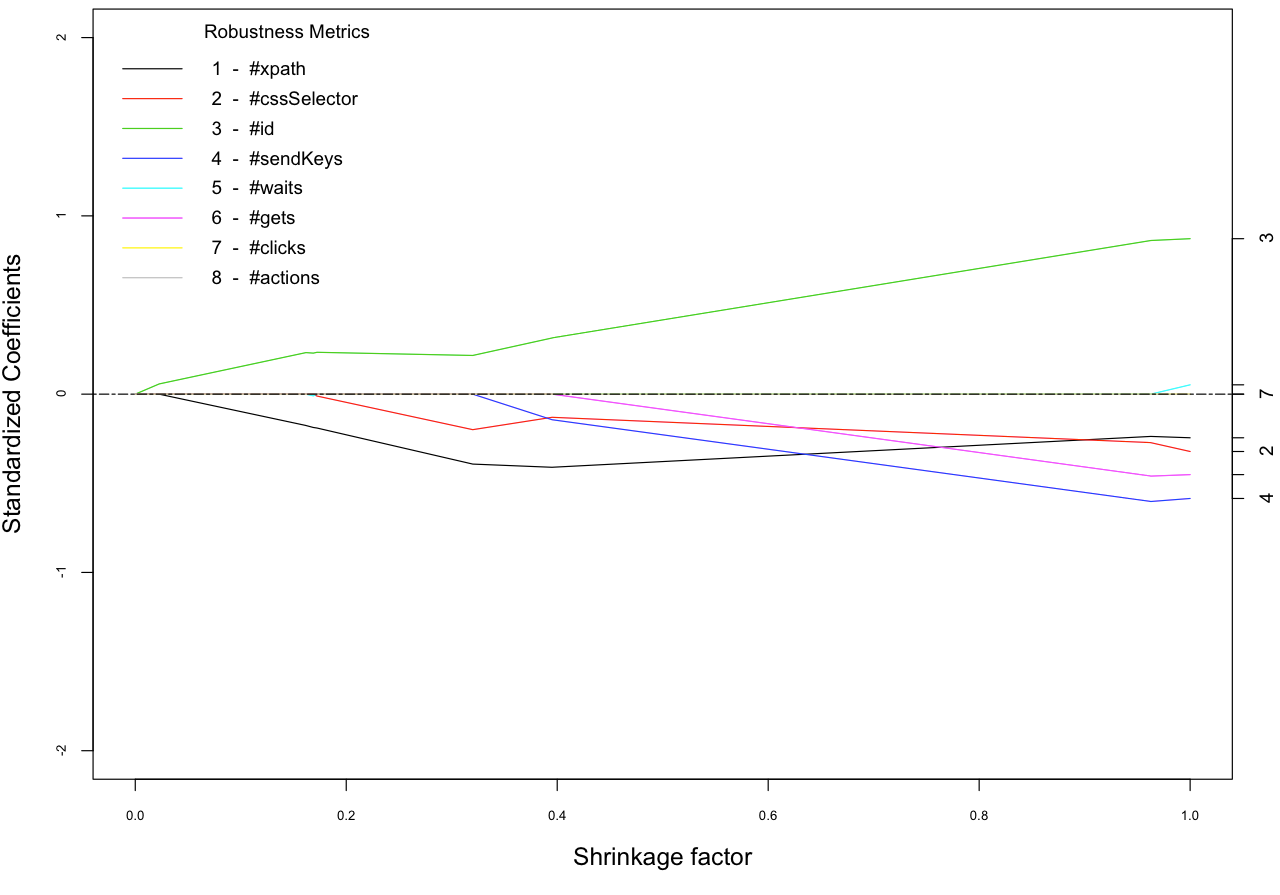
\includegraphics[width=13cm,height=10cm]{./Figures/moodlelasso}}
  \captionsetup{justification=justified,
singlelinecheck=false}
\caption{The \textit{lasso} shrinkage model for Moodle. The x-axis represents the shrinkage estimation and the y-axis represents standardized correlation coefficients. The legend on the top-left corner represents the robustness metrics.}
\label{fig:lasso1}
\end{figure} 

\begin{figure}[ht!] 
\centering     %%% not \center
\subfigure[Mozilla Marketplace]{\label{fig:fireplacelasso}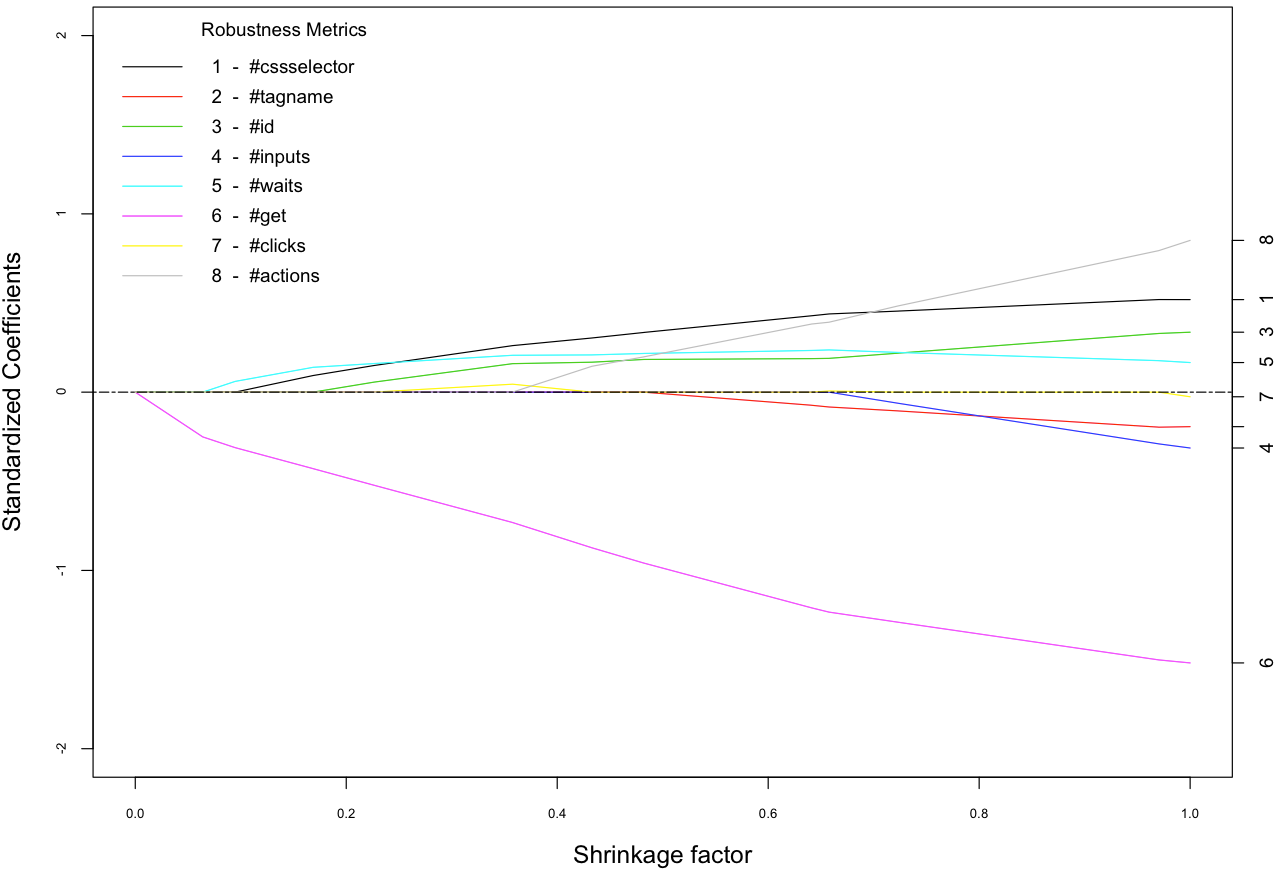
\includegraphics[width=13cm,height=10cm]{./Figures/fireplacelasso}}
\subfigure[Mozilla Addons]{\label{fig:amolasso}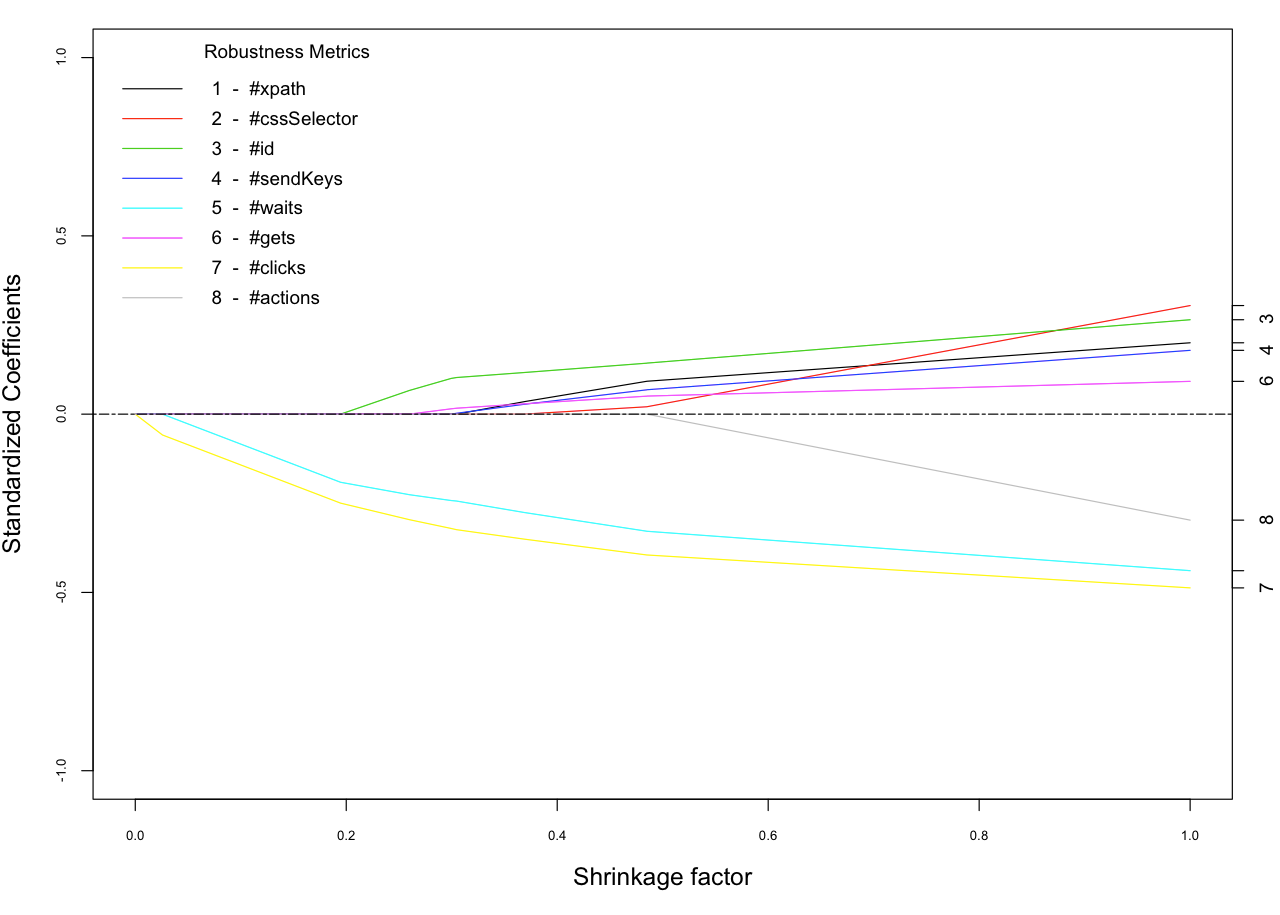
\includegraphics[width=13cm,height=10cm]{./Figures/amolasso}}
  \captionsetup{justification=justified,
singlelinecheck=false}
\caption{The \textit{lasso} shrinkage models for Mozilla Marketplace and Mozilla Addons. The x-axis represents the shrinkage estimation and the y-axis represents standardized correlation coefficients. The legend on the top-left corner represents the robustness metrics. }
\label{fig:lasso2}
\end{figure} 

\begin{figure}[ht!] 
\centering     %%% not \center
\subfigure[Jenkins]{\label{fig:jenkinslasso}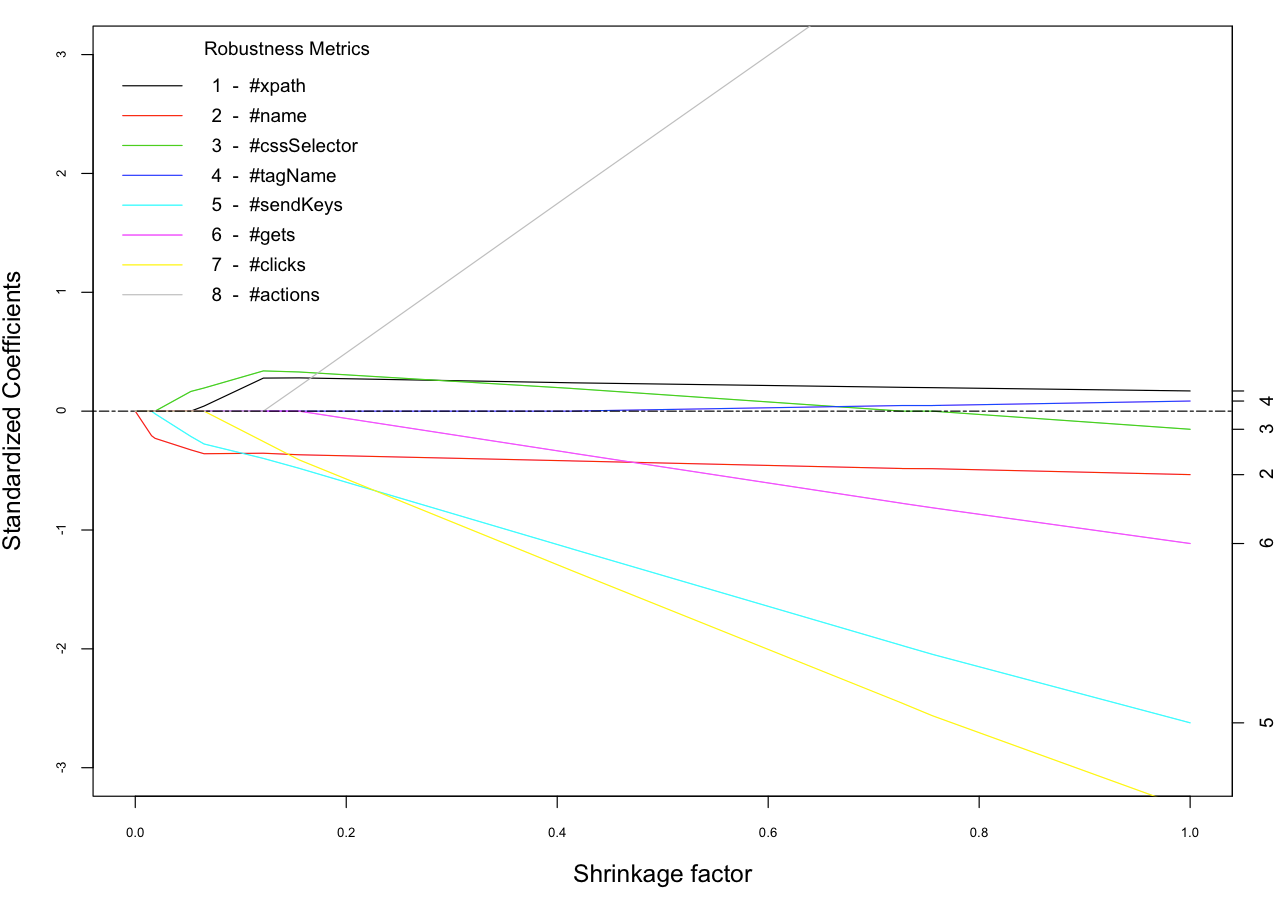
\includegraphics[width=13cm,height=10cm]{./Figures/jenkins}}
\subfigure[Mozilla.org]{\label{fig:bedrocklasso}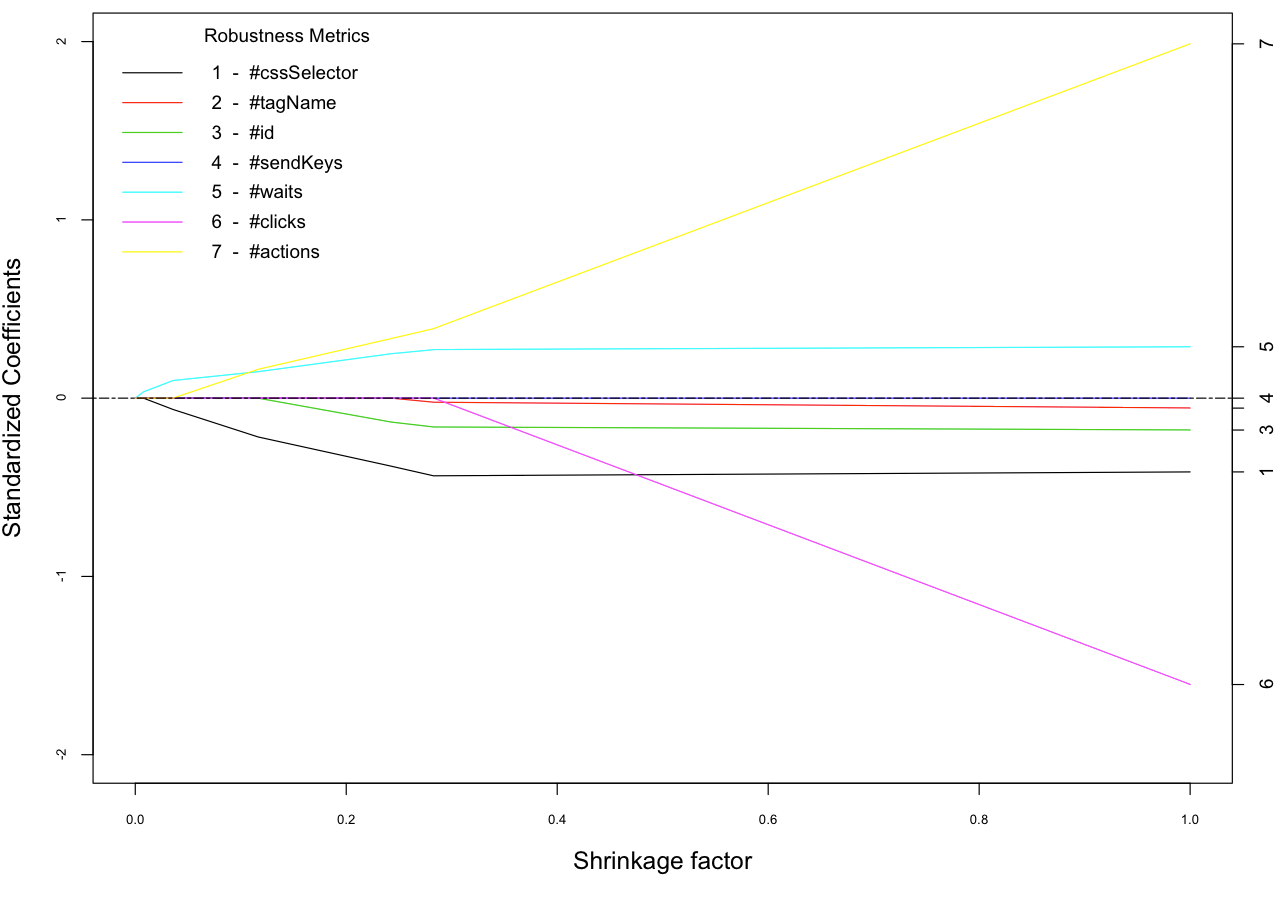
\includegraphics[width=13cm,height=10cm]{./Figures/bedrocklasso}}
  \captionsetup{justification=justified,
singlelinecheck=false}
\caption{The \textit{lasso} shrinkage models for Jenkins and Mozilla.org. The x-axis represents the shrinkage estimation and the y-axis represents standardized correlation coefficients. The legend on the top-left corner represents the robustness metrics. }
\label{fig:lasso3}
\end{figure} 

